\documentclass[11pt]{article}

% Change "review" to "final" to generate the final (sometimes called camera-ready) version.
% Change to "preprint" to generate a non-anonymous version with page numbers.
\usepackage[review]{acl}

% Standard package includes
\usepackage{times}
\usepackage{latexsym}
\usepackage{xcolor}
\usepackage{colortbl}
\usepackage{subcaption}

% For proper rendering and hyphenation of words containing Latin characters (including in bib files)
\usepackage[T1]{fontenc}
% For Vietnamese characters
% \usepackage[T5]{fontenc}
% See https://www.latex-project.org/help/documentation/encguide.pdf for other character sets

% This assumes your files are encoded as UTF8
\usepackage[utf8]{inputenc}

% This is not strictly necessary, and may be commented out,
% but it will improve the layout of the manuscript,
% and will typically save some space.
\usepackage{microtype}
\usepackage{url}
 \usepackage{multirow}


% Standard package includes
\usepackage{times}
\usepackage{latexsym}
\usepackage{enumitem}
\usepackage{listings}
\usepackage{url}
% For proper rendering and hyphenation of words containing Latin characters (including in bib files)
\usepackage[T1]{fontenc}
% For Vietnamese characters
% \usepackage[T5]{fontenc}
% See https://www.latex-project.org/help/documentation/encguide.pdf for other character sets

% This assumes your files are encoded as UTF8
\usepackage[utf8]{inputenc}

% This is not strictly necessary, and may be commented out.
% However, it will improve the layout of the manuscript,
% and will typically save some space.
\usepackage{microtype}

% This is also not strictly necessary, and may be commented out.
% However, it will improve the aesthetics of text in
% the typewriter font.
\usepackage{inconsolata}



%% package imports not in default paper template below

\usepackage{longtable}
% is setspace even used? It causes problems with hyperref, apparently needs to be loaded later..
%\usepackage{setspace}
\usepackage{graphicx}

\usepackage{caption}
\usepackage{subcaption}

\usepackage{colortbl}
\usepackage{makecell}
\usepackage{multirow}
\usepackage{supertabular}
\usepackage{placeins}

% \setlength{\tabcolsep}{0pt}   % this was actually supposed to be in block only for transcripts... now all tables will look weird.. FIXME
\usepackage{subfiles}
\usepackage{enumitem}

% maths and pseodocode
\usepackage{algorithm}
\usepackage{algpseudocode}
\usepackage{amsmath}

% references
\usepackage{cleveref}

% use this to format itemize lists
%\setlist[itemize]{align=right,itemindent=1em,labelsep=1em,labelwidth=1em,leftmargin=1em,nosep}
\setlist[itemize]{leftmargin=1em}  % smaller left margin = more text on one line
%\setlist[enumerate]{leftmargin=1.5em}

\usepackage{booktabs}

% all this insane effort just to typset the prompt....
% I am not going to admit how long it took me to create this...
\usepackage{tcolorbox}
\newcounter{promptno}[section]
\newlength\mystoreparindent
\newenvironment{prompt}[1][]
{
  \setlength{\mystoreparindent}{\the\parindent}
  \setlength{\parindent}{0pt}
  \refstepcounter{promptno}
  \par\medskip
  \noindent
  \begin{tcolorbox}[left=1pt,right=1pt]
%  \textsc{prompt~{\small\thesubsection.\thepromptno}}\\
  \textsc{{template \small\thesubsection.\thepromptno}}\\
  \small
  \tt
}{
  \end{tcolorbox}
  \setlength{\parindent}{\mystoreparindent}
  \medskip
}

\newcounter{utterance}
\usepackage{amssymb}

\usepackage{color}
\newcommand{\das}[1]{\textcolor{red}{//David: #1//}}

\newcommand{\tk}[1]{\textcolor{teal}{//Tim-Kristina: #1//}}
\newcommand{\kr}[1]{\textcolor{orange}{//Karl-Ruilin: #1//}}
\newcommand{\roland}[1]{\textcolor{brown}{//Roland: #1//}}
\newcommand{\rb}[1]{\textcolor{purple}{//Raffella: #1//}}

% define a new column type for model names
\newcolumntype{T}{>{\ttfamily}l}

\newcommand{\model}[1]{\texttt{#1}}



% Defining the dialogue bubbles

% using numbering from https://tex.stackexchange.com/questions/290656/numbering-of-tcolorbox
\tcbuselibrary{skins}
\newcounter{nbubbles}

\definecolor{a-colour}{RGB}{135,74,175}
\definecolor{b-colour}{RGB}{243,145,9}
\definecolor{gm-colour}{RGB}{128,128,128}
\definecolor{wordlegreen}{rgb}{0.4,0.79,0.17}
\definecolor{wordlered}{rgb}{0.86,0.31,0.29}
\definecolor{wordleyellow}{rgb}{1,1,0}


\def \dcolwidth {3cm}
\def \skipcolwidth {0.8cm}
\def \arccorner {3mm}
\def \disttocorner {6pt}

\newtcolorbox[use counter=nbubbles]{a-gm}[1]{
    colback=a-colour!10!white,
    colframe=a-colour,
    fonttitle=\bfseries\tiny,
    fontupper=\footnotesize,
    title={#1},
    sharp corners=west,
    arc=\arccorner,
    width=\dcolwidth,
    left skip=0cm,
    top=0pt,
    bottom=0pt,
    left=0pt,
    right=\disttocorner,
    before={\vspace{-0.1cm}},
    boxrule=0.5pt,
    enhanced,
    attach boxed title to top left={yshift=-0.1mm},
    boxed title style={size=small,colback=a-colour},
    overlay unbroken and first = {
    \node[text width=0.4cm,draw=black,line width=0.1mm,align=center,gray] at (-0.5,0.2) {\footnotesize \thetcbcounter};
  }
}

\newtcolorbox[use counter=nbubbles]{gm-a}[1]{
    colback=gm-colour!5!white,
    colframe=gm-colour,
    fonttitle=\bfseries\tiny,
    fontupper=\footnotesize,
    title={#1},
    sharp corners=east,
    arc=\arccorner,
    width=\dcolwidth + \skipcolwidth,
    left skip=\skipcolwidth,
    top=0pt,
    bottom=0pt,
    left=\disttocorner,
    right=0pt,
    before={\vspace{-0.1cm}},
    boxrule=0.5pt,
    halign title=flush right,
    enhanced,
    attach boxed title to top right={yshift=-0.1mm},
    boxed title style={size=small,colback=gm-colour},
    overlay unbroken and first = {
    \node[anchor=north east,text width=0.4cm,draw=black,line width=0.1mm,align=center,gray] at (-0.9,0.55) {\footnotesize\thetcbcounter};}
}

\newtcolorbox[use counter=nbubbles]{b-gm}[1]{
    colback=b-colour!10!white,
    colframe=b-colour,
    fonttitle=\bfseries\tiny,
    fontupper=\footnotesize,
    title={#1},
    sharp corners=east,
    arc=\arccorner,
    width=\dcolwidth + \skipcolwidth + \dcolwidth +  \skipcolwidth,
    left skip=\dcolwidth + \skipcolwidth + \skipcolwidth,
    top=0pt,
    bottom=0pt,
    left=\disttocorner,
    right=0pt,
    before={\vspace{-0.1cm}},
    boxrule=0.5pt,
    halign title=flush right,
    % boxed title
    enhanced,
    attach boxed title to top right={yshift=-0.1mm},
    boxed title style={size=small,colback=b-colour},
    overlay unbroken and first = {
    \node[anchor=north east,text width=0.4cm,draw=black,line width=0.1mm,align=center,gray] at (-4.7,0.55) {\footnotesize\thetcbcounter};}
}

\newtcolorbox[use counter=nbubbles]{gm-b}[1]{
    colback=gm-colour!5!white,
    colframe=gm-colour,
    fonttitle=\bfseries\tiny,
    fontupper=\footnotesize,
    title={#1},
    sharp corners=west,
    arc=\arccorner,
    width=\dcolwidth + \skipcolwidth + \dcolwidth,
    left skip=\dcolwidth + \skipcolwidth,
    top=0pt,
    bottom=0pt,
    left=0pt,
    right=\disttocorner,
    before={\vspace{-0.1cm}},
    boxrule=0.5pt,
    enhanced,
    attach boxed title to top left={yshift=-0.1mm},
    boxed title style={size=small,colback=gm-colour},
    overlay unbroken and first = {
    \node[anchor=north east,text width=0.4cm,draw=black,line width=0.1mm,align=center,gray] at (-3.9,0.55) {\footnotesize\thetcbcounter};}
}

\newtcolorbox[use counter=nbubbles]{gm-gm}[1]{
    colback=gm-colour!5!white,
    colframe=gm-colour,
    fonttitle=\bfseries\tiny,
    fontupper=\footnotesize,
    title={#1},
    sharp corners,
    width=\dcolwidth + \dcolwidth + \skipcolwidth + \skipcolwidth,
    leftright skip=\dcolwidth,
    top=0pt,
    bottom=0pt,
    left=0pt,
    right=0pt,
    before={\vspace{-0.1cm}},
    boxrule=0.5pt,
    halign title=center,
    enhanced,
    attach boxed title to top center={yshift=-0.1mm},
    boxed title style={size=small,colback=gm-colour},
    overlay unbroken and first = {
    \node[anchor=north east,text width=0.4cm,draw=black,line width=0.1mm,align=center,gray] at (-3.1,0.55) {\footnotesize\thetcbcounter};}
}

%%% end of bubbles definition


% This is also not strictly necessary, and may be commented out.
% However, it will improve the aesthetics of text in
% the typewriter font.
\usepackage{inconsolata}

%Including images in your LaTeX document requires adding
%additional package(s)
\usepackage{graphicx}

% If the title and author information does not fit in the area allocated, uncomment the following
%
%\setlength\titlebox{<dim>}
%
% and set <dim> to something 5cm or larger.

\title{The Price of Thought: A Multilingual Analysis of Reasoning, Performance, and Cost of Negotiation in Large Language Models}



% Author information can be set in various styles:
% For several authors from the same institution:
% \author{Author 1 \and ... \and Author n \\
%         Address line \\ ... \\ Address line}
% if the names do not fit well on one line use
%         Author 1 \\ {\bf Author 2} \\ ... \\ {\bf Author n} \\
% For authors from different institutions:
% \author{Author 1 \\ Address line \\  ... \\ Address line
%         \And  ... \And
%         Author n \\ Address line \\ ... \\ Address line}
% To start a separate ``row'' of authors use \AND, as in
% \author{Author 1 \\ Address line \\  ... \\ Address line
%         \AND
%         Author 2 \\ Address line \\ ... \\ Address line \And
%         Author 3 \\ Address line \\ ... \\ Address line}

\author{First Author \\
  Affiliation / Address line 1 \\
  Affiliation / Address line 2 \\
  Affiliation / Address line 3 \\
  \texttt{email@domain} \\\And
  Second Author \\
  Affiliation / Address line 1 \\
  Affiliation / Address line 2 \\
  Affiliation / Address line 3 \\
  \texttt{email@domain} \\}

%\author{
%  \textbf{First Author\textsuperscript{1}},
%  \textbf{Second Author\textsuperscript{1,2}},
%  \textbf{Third T. Author\textsuperscript{1}},
%  \textbf{Fourth Author\textsuperscript{1}},
%\\
%  \textbf{Fifth Author\textsuperscript{1,2}},
%  \textbf{Sixth Author\textsuperscript{1}},
%  \textbf{Seventh Author\textsuperscript{1}},
%  \textbf{Eighth Author \textsuperscript{1,2,3,4}},
%\\
%  \textbf{Ninth Author\textsuperscript{1}},
%  \textbf{Tenth Author\textsuperscript{1}},
%  \textbf{Eleventh E. Author\textsuperscript{1,2,3,4,5}},
%  \textbf{Twelfth Author\textsuperscript{1}},
%\\
%  \textbf{Thirteenth Author\textsuperscript{3}},
%  \textbf{Fourteenth F. Author\textsuperscript{2,4}},
%  \textbf{Fifteenth Author\textsuperscript{1}},
%  \textbf{Sixteenth Author\textsuperscript{1}},
%\\
%  \textbf{Seventeenth S. Author\textsuperscript{4,5}},
%  \textbf{Eighteenth Author\textsuperscript{3,4}},
%  \textbf{Nineteenth N. Author\textsuperscript{2,5}},
%  \textbf{Twentieth Author\textsuperscript{1}}
%\\
%\\
%  \textsuperscript{1}Affiliation 1,
%  \textsuperscript{2}Affiliation 2,
%  \textsuperscript{3}Affiliation 3,
%  \textsuperscript{4}Affiliation 4,
%  \textsuperscript{5}Affiliation 5
%\\
%  \small{
%    \textbf{Correspondence:} \href{mailto:email@domain}{email@domain}
%  }
%}

\begin{document}
\maketitle
\begin{abstract}
This document is a supplements to the general instructions for *ACL authors. It contains instructions for using the \LaTeX{} style files for ACL conferences.
The document itself conforms to its own specifications, and is therefore an example of what your manuscript should look like.
These instructions should be used both for papers submitted for review and for final versions of accepted papers.
\end{abstract}

\section{Introduction}

Negotiation is a key aspect of human social and economic behaviour that poses significant challenges for AI systems. The problem is complex - agents must produce coherent language while performing strategic reasoning, modelling opponent preferences and goals, and managing the tension between cooperation and competition to maximize outcomes. With LLMs increasingly being being deployed as autonomous agents in domains ranging from e-commerce to resource distribution, negotiation capability has become essential. Negotiation tasks therefore provide a strong test-bed for measuring agent competence, offering interactive, multi-turn scenarios with objective success measures that go beyond static evaluation and test integrated capabilities from language understanding to theory of mind.


Recent work has systematically assessed LLM negotiation performance, uncovering varied emergent behaviors and notable weaknesses. Studies consistently show that LLMs often deviate from optimal game-theoretic play, with unreliable performance across tasks (Hua et al. 2024; Bianchi et al. 2024). While larger proprietary models typically outperform smaller ones, even top-performing systems can lose to weaker opponents and fail in cooperative scenarios (Davidson et al. 2024; Kwon et al. 2024). These models can acquire complex deceptive tactics like expressing false interest in low-value items for later concessions (Lewis et al. 2017). Yet they also exhibit cognitive biases such as anchoring effects and respond to social signals - counterintuitively, expressing desperation can improve outcomes (Bianchi et al. 2024). Despite these capabilities, serious limitations remain. LLMs show clear asymmetries, performing much worse as buyers than sellers (Xia et al. 2024). Their behavioral failures create real economic risks: budget violations, overpayment, and negotiation breakdowns (Zhu et al. 2025). Current approaches attempt to address these issues through structured, game-theoretic frameworks that constrain agent behavior and improve decision quality (Hua et al. 2024).

\section{Related Work}

\cite{DBLP:journals/corr/abs-2402-01704} 

\cite{DBLP:journals/corr/abs-2503-06416}

\cite{DBLP:journals/corr/abs-2505-07775}

\cite{DBLP:conf/emnlp/Shea024}

\cite{sun2025gametheorymeetslarge}

\cite{DBLP:conf/sigdial/JeknicSK24} (clean up)

\cite{DBLP:journals/corr/abs-2011-01975} (clean up)

\cite{DBLP:conf/icml/0001CYTJ024} (negotiation arena)

\cite{DBLP:journals/corr/LewisYDPB17} ( deal or no deal)

\cite{DBLP:conf/iclr/DavidsonVK024}

\cite{DBLP:journals/corr/abs-2411-05990}

\cite{DBLP:conf/emnlp/KwonWKCLG24}

\cite{DBLP:conf/acl/Xia0RMZ0024}

\cite{DBLP:journals/corr/abs-2506-00073}

\cite{esfandiari-baiat-edlund-2024-meet} (air balloon)

% previous attempts at negotiation abilities - before LLM era
% current papers with LLMs
% missing points etc.


%%% Cleann Up



%%%% Deal or no deal


%%%% Air Balloon Survival - personal preferences

\section{Dialogue Games for Evaluating Negotiation Abilities}

clembench description bla bla bla~\cite{chalamalasetti-etal-2023-clembench}

% why dialogue games are good for this

%%% The general idea of the game - what is it measuring

\subsection{Deal or No Deal}

% \roland{Game descriptions etc.}

% \cite{DBLP:journals/corr/LewisYDPB17}

%%% The general idea of the game - what is it measuring, why is it a viable game for measuring negotiation.... - motivation for the game

The Deal or No Deal (DoND) game is a two-player, turn-based dialogue game designed to simulate a multi-issue bargaining scenario. \Cref{fig:dond_example} shows a synthetic example of a successfully played episode of the game. DoND has previously been proposed in \cite{DBLP:journals/corr/LewisYDPB17} to training an AI system for negotiation. More recently, \cite{DBLP:journals/corr/abs-2406-18872} used the same DoND game and proposed three different variations, two of which are used in this work.
In DoND, players must communicate to reach a mutually beneficial agreement on the division of a set of items, each holding different values for each player. The game tries to evaluate negotiation skills, ability to express and understand preferences, and the ability to compromise. Aside from negotiation, the game also challenges the ability of LLMs to adhere to rules, such as using a specific syntax for final proposals.

% one figure that shows sample transcript and how the players interact etc. - take a look at Fig 1 in here: https://aclanthology.org/2025.coling-main.381.pdf

\begin{figure}[ht]
  \centering
  {
\scriptsize
\setcounter{utterance}{1}
\setlength{\tabcolsep}{0pt}
\begin{supertabular}{c@{$\;$}|p{.15\linewidth}@{}p{.15\linewidth}p{.15\linewidth}p{.15\linewidth}p{.15\linewidth}p{.15\linewidth}}   
  \# & $\;$\textbf{Player A} & \multicolumn{4}{c}{\textbf{Game Master}} & $\;\:$\textbf{Player B}\\
  \hline

  \theutterance \stepcounter{utterance} & &
  \multicolumn{4}{p{0.6\linewidth}}{
    \cellcolor[rgb]{0.9,0.9,0.9}{
      \makecell[{{p{\linewidth}}}]{
        \tt {\tiny [A$\langle$GM$\rangle$B]}
        <GAME DESCRIPTION> ... \\
        \tt Available items: 1 book, 2 hats, 2 balls.
      }
    }
  } & \\

  \theutterance \stepcounter{utterance} & &
  \multicolumn{4}{p{0.6\linewidth}}{
    \cellcolor[rgb]{0.9,0.9,0.9}{
      \makecell[{{p{\linewidth}}}]{
        \tt {\tiny [A$\langle$GM]}
        \tt Player A value function: book: 0,\\ \tt hat: 1, ball: 4.
      }
    }
  }  \vspace{0.55em} & \\
 
  \theutterance \stepcounter{utterance} & &
  \multicolumn{4}{p{0.6\linewidth}}{
    \cellcolor[rgb]{0.9,0.9,0.9}{
      \makecell[{{p{\linewidth}}}]{
        \tt {\tiny [GM$\rangle$B]}
        \tt Player B value function: book: 6,\\ \tt hat: 1, ball: 1.
      }
    }
  } & \\

  \theutterance \stepcounter{utterance} &
  \multicolumn{4}{p{0.6\linewidth}}{
    \cellcolor[rgb]{0.8,1,0.9}{
      \makecell[{{p{\linewidth}}}]{
        \tt {\tiny [A$\rangle$B]}
        Hi! Here are my preferences: I value balls the most, then hats, and I don't value the book at all. How about you? What do you value most? 
      }
    } 
  } & & \\
 
  \theutterance \stepcounter{utterance} & & &
  \multicolumn{4}{p{0.6\linewidth}}{
    \cellcolor[rgb]{1,0.85,0.72}{
      \makecell[{{p{\linewidth}}}]{
        \tt {\tiny [A$\langle$B]}
        Thanks for sharing! I value the book most, while hats and balls are equally less important to me. Would you take both balls and one hat, and I'll take the book and the other hat? That way, we both get what we value most.
      }
    }
  } \\
 
  \theutterance \stepcounter{utterance} &
  \multicolumn{4}{p{0.6\linewidth}}{
    \cellcolor[rgb]{0.8,1,0.9}{
      \makecell[{{p{\linewidth}}}]{
        \tt {\tiny [A$\rangle$B]}
        That sounds fair! With this split, I'd get both balls and one hat, while you'd get the book and one hat, so we each get what we value most. Ready to submit this as my proposal unless you'd like to tweak anything.
      }
    }
  } & & \\
 
  \theutterance \stepcounter{utterance} & & &
  \multicolumn{4}{p{0.6\linewidth}}{
    \cellcolor[rgb]{1,0.85,0.72}{
      \makecell[{{p{\linewidth}}}]{
        \tt {\tiny [A$\langle$B]}
        I agree with the split. I'll take the book and one hat, you take both balls and the other hat.
      }
    } 
  } \\
 
  \theutterance \stepcounter{utterance} &
  \multicolumn{4}{p{0.6\linewidth}}{
    \cellcolor[rgb]{0.8,1,0.9}{
      \makecell[{{p{\linewidth}}}]{
        \tt {\tiny [A$\rangle$GM]}
        [Proposal: 1 hat, 2 balls] 
      }
    }
  } & & \\
 
  \theutterance \stepcounter{utterance} & &
  \multicolumn{4}{p{0.6\linewidth}}{
    \cellcolor[rgb]{0.9,0.9,0.9}{
      \makecell[{{p{\linewidth}}}]{
        \tt {\tiny [GM$\rangle$B]}  
        The other player has submitted a proposal. You must now submit your proposal.
      }
    }
  } & \\

  \theutterance \stepcounter{utterance} & & &
  \multicolumn{4}{p{0.6\linewidth}}{
    \cellcolor[rgb]{1,0.85,0.72}{
      \makecell[{{p{\linewidth}}}]{
        \tt {\tiny [GM$\langle$B]}  
        [Proposal: 1 book, 1 hat] 
      }
    }
  } \\
\end{supertabular}
}

  \caption{Synthetic example of a DoND game episode. Note that the initial prompts given by the game master have been truncated for brevity. The game ends in a successful Pareto optimal agreement.}
  \label{fig:dond_example}
\end{figure}

%%% IMplementation details: explain the game dynamics - 2 player etc., instances,

\paragraph{Game Mechanics}

At the start of each game, players are presented with a shared set of items, consisting of several types and quantities. In addition to the shared set of items, each player is also secretly given a different value function, mapping each item type to a non-negative integer indicating how much the player values that specific type of item. The fact that the two players value functions are different creates the central conflict in the game.

After having received the initial prompt from the game master, containing the rules of the game, the shared set of items, and the players respective set of items, players are able to exchange free-form natural language messages. These messages are transmitted directly between the players and can be in any format, provided they do not contain the special proposal syntax. This enables the players to engage in negotiation about how to divide the items, with the goal of reaching an agreement.

At any point during the conversation, or once prompted to by the game master after a turn limit is reached, the players can make a secret proposal using a specific syntax. Once one player has made a proposal, the game master instructs the other player to also make a proposal, crucially however, without revealing the content of the first proposal.

After both proposals are submitted, the game can end in either of two outcomes. Either the proposals are compatible, i.e., there are enough items to satisfy both proposals, or the proposals are conflicting. In case of compatible proposals, each player is awarded points based on total value of items they requested, according to their private value function. Should the proposals be conflicting, however, both players receive zero points.

The game master strictly enforces the rules. If a player fails to follow instructions, the game is immediately aborted. Unlike in \cite{DBLP:journals/corr/abs-2406-18872} there is no re-prompting on errors, making rule adherence a critical component of successful play.

%%% Experiments: details of the experiments & number of instances etc.

\paragraph{Instance Generation}

The game instances for the evaluation were generated programmatically, ensuring a wide variety for possible initial conditions and controlled difficulty. Each instance was generated with a maximum turn limit of 5 and each game instance features a random set of between 3 and 5 different item types. The item types for each game have been randomly sampled from a predefined list of 100 common nouns. The total number of items was set to between 5 and 8, with every item type being present at least once and the remaining capacity being randomly distributed among the item types. Finally, a random value function of non-negative integers for all item types was generated for each player.

The value functions were generated subject to the same constraints as in previous work on DoND \cite{DBLP:journals/corr/abs-2406-18872,DBLP:journals/corr/LewisYDPB17}. The maximum value a single player can achieve by receiving all the items in the game instance is exactly 10. Every item in the game instance has a non-zero value to at least one of the two players. And lastly, there exists at least one item that has a non-zero value to both players.
These constraints are crucial for creating meaningful negotiation scenarios. The fixed maximum score keeps the value scale consistent, while the two other constraints on the value function ensure that no items are irrelevant and that it is impossible for both players to simultaneously achieve their maximum score, thus forcing a compromise.

Two of the three different game modes proposed in \cite{DBLP:journals/corr/abs-2406-18872} have been evaluated. The initial prompt given to the players is identical across modes, except for the final rule which specifies the optimization objective to the players.
In the \textbf{semi-competitive} mode, players are asked to maximize their own score. This is the standard negotiation setting, and it requires players to balance cooperation, to avoid zero-point conflicts, with competition, to maximize their individual share.
For the \textbf{cooperative} mode of the game, players are asked to maximize the sum of both players scores. This transforms the game into a purely cooperative task, in which two rational agents should always achieve the maximum score, assuming they are able to communicate and reason about the preferences perfectly.

\paragraph{Evaluation Metrics}

In addition to the percentage of non-aborted games, the performance of players in the DoND game is also evaluated based on the scores achieved by the players.
For the cooperative game mode, assessing the quality of agreement is straightforward. Since both players try to optimize for the same total score of both players, it is sufficient to use the ratio between the achieved total score to the maximum total score for that game instance, $\mathit{Quality}_\mathit{coop} = \frac{\mathit{Score}_A + \mathit{Score}_B}{\max ( \mathit{Score}_A' + \mathit{Score}_B' )}$.

Evaluating the game in the semi-competitive setting is slightly more involved, as it requires finding a single score that jointly reflects the quality of the outcome for both players. For this, a metric based on Pareto efficiency has been used. The score is defined as one minus the normalized maximum possible Pareto improvement, $\mathit{Quality}_\mathit{semi} = 1 - \frac{\mathit{Maximum Pareto Improvement}}{\max ( \mathit{Score}_i' )}$. The maximum possible Pareto improvement is the largest amount the score of one player could be increased without decreasing the score of the other. Normalization is performed by dividing by the maximum score a single player can obtain.

\subsection{Clean Up}

Clean Up is a turn-based dialogue game for two players focussed on cooperative strategy development and object rearrangement. Both players are presented with identical $7\times7$ ASCII-like grids, with a number of randomly distributed objects in the form of capital letters placed on them. Placement is different for each player and each player can only see their own grid, cf.~\cref{fig:clean_up_example}. The goal is to rearrange the objects in such away that their respective positions match across both grids. Scoring is based on the Euclidean distance of the identical objects on both grids.

Object rearrangement has been a long standing challenge in the field of artificial intelligence requiring understanding of the given situation, the action space, and spatial reasoning, cf.~\citet{DBLP:journals/corr/abs-2011-01975}, \citet{DBLP:journals/ral/ZengWYZDCD24}, \citet{DBLP:journals/access/KhanQCASR25}.

Collaborative reconstruction games, where one player knows the desired target state and has to instruct their counterpart to recreate it, have been extensively studied (see \citet{DBLP:journals/jair/SugliaKL24} for an overview). In this game, however, the players are on par and need to both negotiate their common goal state and a strategy of reaching it (cf.~\citet{DBLP:conf/sigdial/JeknicSK24}, which examines human-human and human-computer interaction in a similar game).

\begin{figure}[ht!]
    \centering
    % \newcounter{utterance}

\footnotesize  \setcounter{utterance}{1}
\setlength{\tabcolsep}{0pt}
\begin{supertabular}{c@{$\;$}|p{.15\linewidth}@{}p{.15\linewidth}p{.15\linewidth}p{.15\linewidth}p{.15\linewidth}p{.15\linewidth}}   
\# & $\;$A & \multicolumn{4}{c}{Game Master} & $\;\:$B\\
    \hline

\theutterance \stepcounter{utterance}  
    & & \multicolumn{4}{p{0.6\linewidth}}{
        \cellcolor[rgb]{0.9,0.9,0.9}{
            \makecell[{{p{\linewidth}}}]{
                \texttt{\tiny{[P1$\langle$GM]}}
                {<GAME DESCRIPTION>}\\
                \centering
                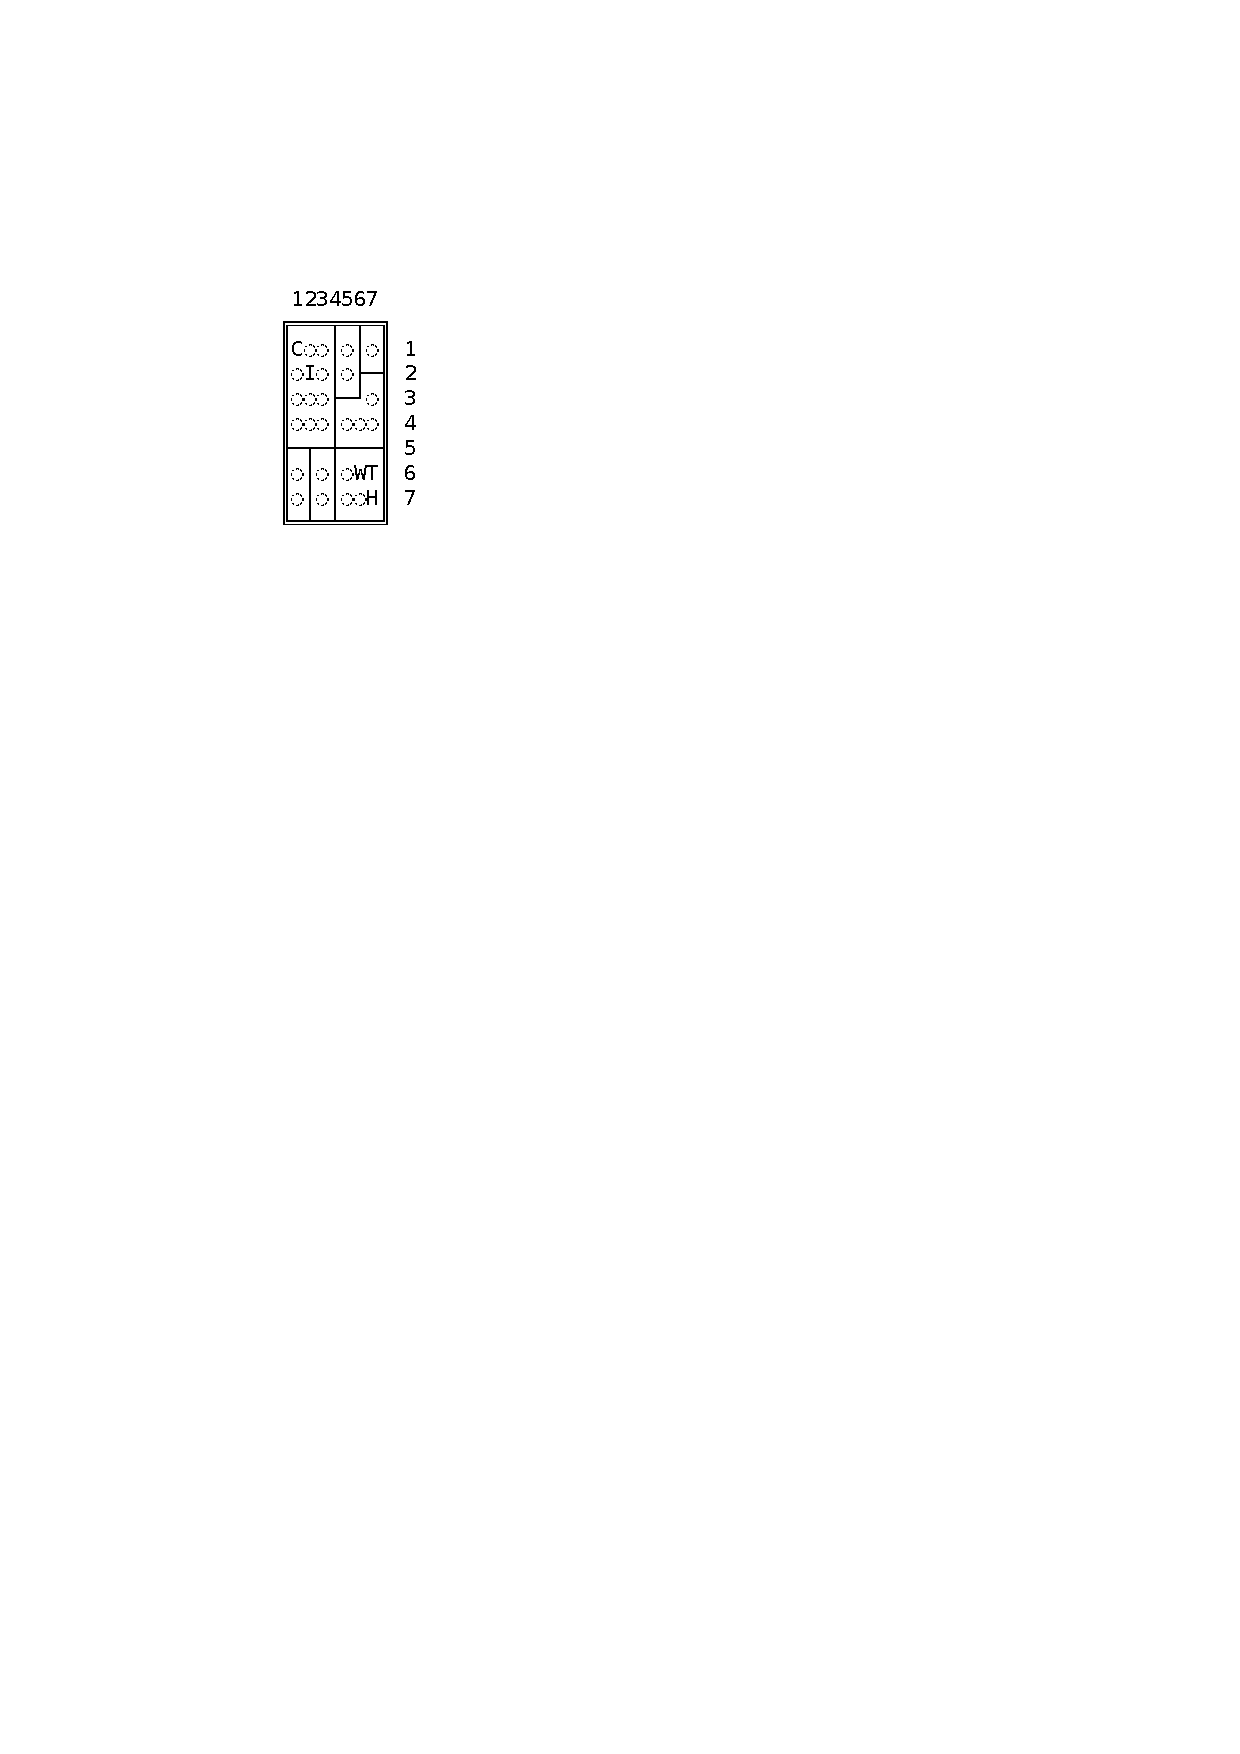
\includegraphics[height=60pt]{clean_up/grid_1_min.pdf}\\
                \raggedright
                \texttt{Please send a message to the other player to start the game!}
            }
        }
    }
    & \\

\theutterance \stepcounter{utterance}  
    & \multicolumn{4}{p{0.6\linewidth}}{
        \cellcolor[rgb]{0.561,0.737,0.561}{
            \makecell[{{p{\linewidth}}}]{
                \texttt{\tiny{[P1$\rangle$GM]}}
                \texttt{SAY: Hi! Let's coordinate our moves. [...]}
            }
        }
    }
    & & \\

\theutterance \stepcounter{utterance}  
    & & \multicolumn{4}{p{0.6\linewidth}}{
        \cellcolor[rgb]{0.9,0.9,0.9}{
            \makecell[{{p{\linewidth}}}]{
                \texttt{\tiny{[GM$\rangle$P2]}}
                \centering{<GAME DESCRIPTION>}\\
                \centering
                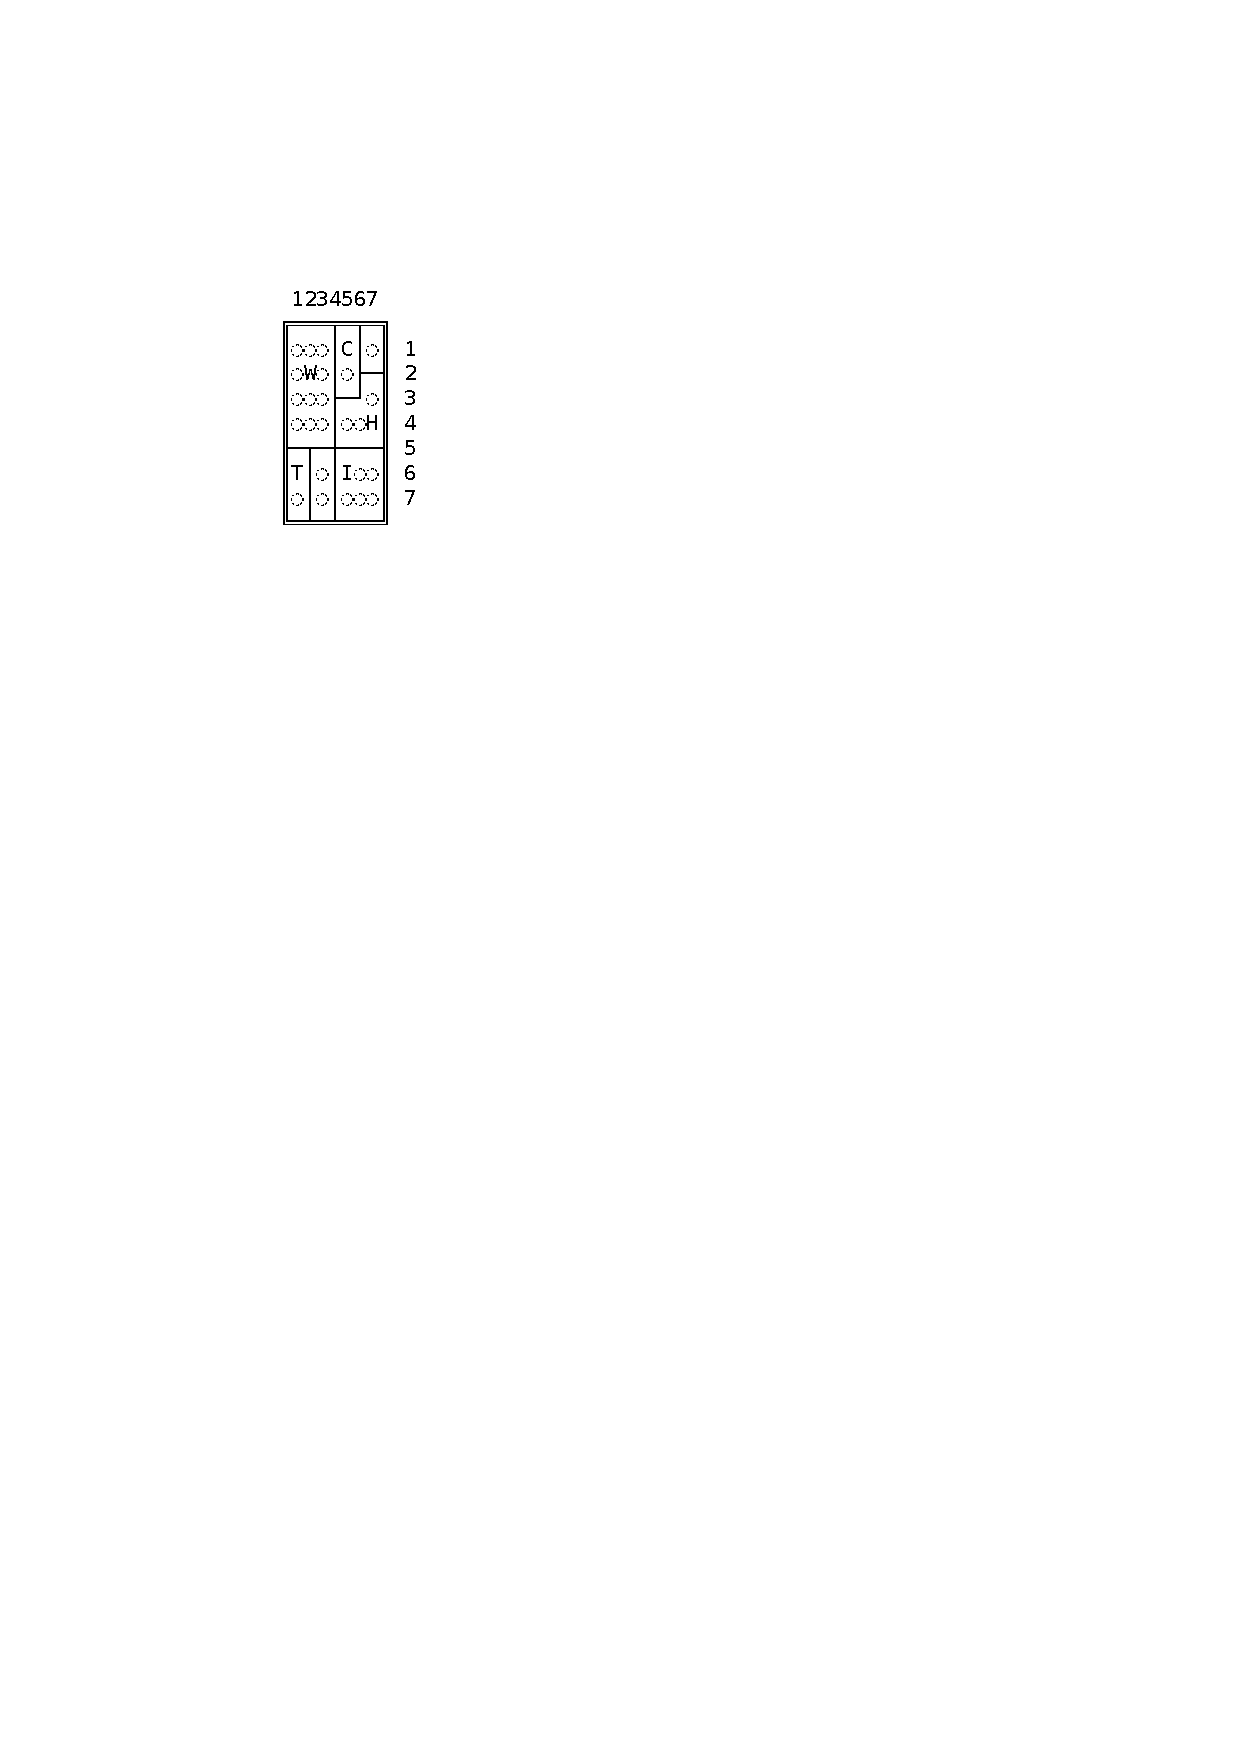
\includegraphics[height=60pt]{clean_up/grid_2_min.pdf}\\
                \raggedright
                \texttt{The other player started the game by sending this message:} \\
                \centering{<MESSAGE>}\\
                \raggedright
                \texttt{What is your first command?}
            }
        }
    }
    & \\

& \multicolumn{6}{c}{
\vdots
} \\

\theutterance \stepcounter{utterance}  
    & & & \multicolumn{4}{p{0.6\linewidth}}{
        \cellcolor[rgb]{0.373,0.62,0.627}{
            \makecell[{{p{\linewidth}}}]{
                \texttt{\tiny{[GM$\langle$P2]}}
                \texttt{MOVE: C, (1,1)} \\
            }
        }
    } \\

\theutterance \stepcounter{utterance}  
    & & \multicolumn{4}{p{0.6\linewidth}}{
        \cellcolor[rgb]{0.9,0.9,0.9}{
            \makecell[{{p{\linewidth}}}]{
                \texttt{\tiny{[P1$\langle$GM]}}
                Your message has been relayed to the other player.\\
                \centering <GAME STATE> \\
                \raggedright
                \texttt{The other player moved an object on their grid. \\What is your next command?}
            }
        }
    }
    & \\
    
\theutterance \stepcounter{utterance}  
    & \multicolumn{4}{p{0.6\linewidth}}{
        \cellcolor[rgb]{0.561,0.737,0.561}{
            \makecell[{{p{\linewidth}}}]{
                \texttt{\tiny{[P1$\rangle$GM]}}
                \texttt{MOVE: I, (5,6)}
            }
        }
    }
    & & \\

& \multicolumn{6}{c}{
    \vdots
} \\
\theutterance \stepcounter{utterance}  
    & & & \multicolumn{4}{p{0.6\linewidth}}{
        \cellcolor[rgb]{0.373,0.62,0.627}{
            \makecell[{{p{\linewidth}}}]{
                \texttt{\tiny{[GM$\langle$P2]}}
                \texttt{SAY: I think our grids are aligned now, finished?} \\
            }
        }
    } \\
\theutterance \stepcounter{utterance}  
    & \multicolumn{4}{p{0.6\linewidth}}{
        \cellcolor[rgb]{0.561,0.737,0.561}{
            \makecell[{{p{\linewidth}}}]{
                \texttt{\tiny{[P1$\rangle$GM]}}
                \texttt{SAY: finished!}
            }
        }
    }
    & & \\
\end{supertabular}
    \caption{Condensed example dialogue from Clean Up. The task is to negotiate a common goal configuration for a number of objects randomly placed on each player`s grid, and move them accordingly. Finally, both players have to agree the goal is reached to end the game. \kr{expand first P1 message}}
    % \vspace*{-.8cm}
    \label{fig:clean_up_example}
\end{figure}

\paragraph{Difficulty Levels and Instances}\label{sec:clean_up_difficulty_levels}  All grids have the same size ($7\times7$), and contain obstacles in form of horizontal and vertical lines, branches, crossings, and corners cf.~\cref{fig:clean_up_example}. They are generated using an ASP encoding to ensure all lines are continuous. We control difficulty along two dimensions: number of empty cells and number of objects.

More empty cells means it's less likely that players try to place objects in occupied cells. Of the 49 total cells, $34$ or $69.4\%$ of cells are empty on the \textit{easy} level, $29$ or $59.2\%$ on \textit{medium}, and $24$ or $49.0\%$ on \textit{hard} (cf.~\cref{clean_up:grid_examples} in \cref{clean_up_exp_setup} for example grids). For each level, we sample three grids, and then place $3$, $5$, or $7$ objects on them, making for $27$ experiments in total.

\paragraph{Game Mechanics} The game is turn based, and the maximum number of rounds is fixed to $4 \times n_{obj}$ (where $n_{obj}$ is the object count). Players can collectively accumulate $2 \times n_{obj} + 2$ penalties.

Initially, P1 (Player~1) is provided with a game description including round and penalty limit and their respective grid, following which they have to send a message to P2 (Player~2). P2 receives the same prompt and P1's message (see~\cref{fig:clean_up_prompt_templates} in \cref{clean_up:prompts} for the full prompt). In each turn, a player can either send a message to their counterpart or move an object on their grid.

Each following turn starts with a message from the Game Master consisting of three parts: (1) feedback on the last turn, i.~e., either a notification that the message has been passed on or the updated grid if they moved an object; (2) information on the game state, i.~e., current and maximum penalties and rounds, and (3) either the other player's message or a notification that they moved an object. 

If a player does not follow the format, tries to move an object to a non-empty space or outside the grid bounds, or tries to move an object that doesn't exist, they receive a penalty and are re-prompted with information on the nature of their mistake. See \cref{fig:clean_up_intermittent_prompts} in \cref{clean_up:prompts} for the full new turn and penalty messages.

The game ends if (1) both players agree to end it, (2) round limit is exceeded, or (3) penalty limit is exceeded.

\paragraph{Evaluation Metrics} A game counts as failure and is not scored if the penalty limit is exceeded. The Quality Score $\mathbf{QS}$ is calculated as follows:
$$\mathbf{QS} = \mathbf{DS} \cdot \mathbf{PS} \cdot 100; \ \mathbf{QS} \in [0, 100]$$

\textbf{Distance Score} $\mathbf{DS} \in [0,1]$ is calculated from three components, each representing the sum of Euclidean distances for all identical objects on both grids: the Initial Distance Sum $\mathbf{I}$ at the start of the game, the Final Distance Sum $\mathbf{F}$ at the end of the game, and the Expected Distance Sum $\mathbb{E}$ that approximates the distances for randomly placed objects (see \cref{clean_up:scoring} for details). The Expected Distance Score $ES$ and Distance Reduction Score $RS$, quantifying how close the players came to the goal of perfect alignment of all objects, are calculated as follows:
\begin{align*}
ES = \max \left\{0,1 - \frac{\mathbf{F}}{\mathbb{E}} \right\}; \
RS = \max \left\{0,1 - \frac{\mathbf{F}}{\mathbf{I}} \right\}
\end{align*}
$\mathbf{DS}$ is then either $0$ if final placement is worse than random, or calculated as the mean of both scores:
\begin{align*}
\mathbf{DS} &= \begin{cases}
\frac{ES+RS}{2} & if \quad ES > 0 \\
0 & otherwise
\end{cases}
\end{align*}

\textbf{Penalty Score} $\mathbf{PS} \in [0.5,1]$ is calculated from the penalty count $P$ normalized against max. penalties $P_m$ as follows:
$$\mathbf{PS} = \frac{P_m}{P-2P_m}+1.5$$
We chose the hyperbolic function because it is lenient for low $P$ and harsher for $P$ close to $P_m$.

%%% The general idea of the game - what is it measuring, why is it a viable game for measuring negotiation.... - motivation for the game

% one figure that shows sample transcript and how the players interact etc. - take a look at Fig 1 in here: https://aclanthology.org/2025.coling-main.381.pdf
 
%%% IMplementation details: explain the game dynamics - 2 player etc., instances,
%%% Experiments: details of the experiments & number of instances etc.

\subsection{Air Balloon Survival}
\textit{Air Balloon Survival} is a conversational negotiation game. Two players are travelling in a sinking hot air balloon and must agree to keep a set of items such that they do not exceed the balloon's maximum weight capacity. Each player is presented with the list of available items and their respective weight. Additionally, both players receive unique preference values for each item which remain hidden from the other player. Players must then negotiate and make a deal which maximizes the utility score, i.e. the sum of preference values of items while respecting the weight constraint. During negotiation, players must respect the rules of the game which include a clear framework governing the syntactic structure of their messages and rules governing which actions they are allowed to take to advance in the game. The game ends once a deal has been made. A deal is defined as an explicit agreement by one player with a proposal their interlocutor has made. A proposal can be any subset of the set of items in the game. A simplified example of an episode can be seen in Figure \ref{fig:air_balloon_example}. \textit{Air Balloon Survival} probes the players abilities to reason and negotiate on two levels. On (1) the level of each individual player and (2) on a collective level. (1) On an individual level, each player is effectively given an instance of a version of the 0/1 Knapsack Problem. Hence, on this individual level our game probes a players ability to perform constraint-based optimization which includes carrying out arithmetic operations and performing combinatorial search over all possible deals. (2) On the collective level, we probe the players’ practical rationality, i.e. their ability to maximize personal utility by successfully negotiating an agreement with their counterpart who may have conflicting goals. Given that players must align by inferring their counterparts’ implicit preferences and intentions from observed responses, the game also connects to the broader topic of Theory of Mind (ToM) and LLMs.
\begin{figure}[ht!]
    \centering
    % \newcounter{utterance}
{\footnotesize  \setcounter{utterance}{1}
\setlength{\tabcolsep}{0pt}
\begin{supertabular}{c@{$\;$}|p{.15\linewidth}@{}p{.15\linewidth}p{.15\linewidth}p{.15\linewidth}p{.15\linewidth}p{.15\linewidth}}   
\# & $\;$A & \multicolumn{4}{c}{Game Master} & $\;\:$B\\
    \hline

\theutterance \stepcounter{utterance}  
    & & \multicolumn{4}{p{0.6\linewidth}}{
        \cellcolor[rgb]{0.9,0.9,0.9}{
            \makecell[{{p{\linewidth}}}]{
                \texttt{\tiny{[A$\langle$GM]}}
                <GAME DESCRIPTION>\\
                \texttt{-Items and weights: Ball(2), Book(3), Magazine(1), Rope(4), Lamp(5)} \\
                \texttt{-Max Weight: 7} \\
                \texttt{-Your Preferences: Ball=1, Book=2, Magazine=2, Rope=2, Lamp=1}
            }
        }
    }
    & \\
    
\theutterance \stepcounter{utterance}  
    & \multicolumn{4}{p{0.6\linewidth}}{
        \cellcolor[rgb]{1,0.9,0.9}{
            \makecell[{{p{\linewidth}}}]{
                \texttt{\tiny{[A$\rangle$GM]}}
                \texttt{PROPOSAL: Magazine, Ball, Book} \\
                \texttt{ARGUMENT: These items balance weight and value well for me. What do you think?}
            }
        }
    }
    & & \\

\theutterance \stepcounter{utterance}  
    & & \multicolumn{4}{p{0.6\linewidth}}{
        \cellcolor[rgb]{0.9,0.9,0.9}{
            \makecell[{{p{\linewidth}}}]{
                \texttt{\tiny{[GM$\rangle$B]}}
                <GAME DESCRIPTION>\\
                \texttt{<Items, weights, weight limit>}\\
                \texttt{-Your Preferences: Ball=1, Book=1, Magazine=2, Rope=4, Lamp=5} \\
                \centering{<PLAYER A Message>}
            }
        }
    }
    & \\

\theutterance \stepcounter{utterance}  
    & & & \multicolumn{4}{p{0.6\linewidth}}{
        \cellcolor[rgb]{0.9,1,0.9}{
            \makecell[{{p{\linewidth}}}]{
                \texttt{\tiny{[GM$\langle$B]}}
                \texttt{PROPOSAL: Rope, Ball, Magazine}\\
                \texttt{ARGUMENT: I value Rope highly, but not Magazine. How about we swap them?}
            }
        }
    } \\

\theutterance \stepcounter{utterance}  
    & & \multicolumn{4}{p{0.6\linewidth}}{
        \cellcolor[rgb]{0.9,0.9,0.9}{
            \makecell[{{p{\linewidth}}}]{
                \texttt{\tiny{[A$\langle$GM]}}
                \centering{<PLAYER B Message>}
            }
        }
    }
    & \\

\theutterance \stepcounter{utterance}  
    & \multicolumn{4}{p{0.6\linewidth}}{
        \cellcolor[rgb]{1,0.9,0.9}{
            \makecell[{{p{\linewidth}}}]{
                \texttt{\tiny{[A$\rangle$GM]}}
                \texttt{AGREE: Rope, Ball, Magazine} \\
                \texttt{ARGUMENT: I am indifferent w.r.t. Rope and Magazine. Fair deal.} \\
            }
        }
    }
    & & \\
    
\end{supertabular}
}
    \caption{A simplified dialogue example from the \textit{Air Balloon Survival} game. In this game, two players must negotiate and argue for their preferred set of items. To reach the goal state, one player must explicitly agree to a proposal made by the other. Messages from player A and player B are shown in red and green, respectively. Grey messages come from the game master, who provides the initial prompts and relays messages between the two players. \tk{I'd say add some made-up list of items and their weights from each player's view so that we see what is there. and they are trying to negotiate for/about etc. Maybe Player 2 could accept some items but negotiate over others based on personal preferences (weights) etc. so that we see how personal preferences play a role here.}}
    \label{fig:air_balloon_example}
\end{figure}
\paragraph{Game Mechanics}
Both players receive initial prompts that may differ in the preference values assigned to items. They are instructed to use specified formats when making proposals and negotiating, and to follow rules such as only being allowed to accept proposals made by the other player (cf. Fig.~\ref{fig:hot_air_balloon_init_prompt} in Appendix~\ref{sec:hot_air_balloon_appendix_prompt_templates}). 
There is no limit on the number of turns, but a game is aborted if no progress is made for eight consecutive turns. Each player may commit up to two mistakes, either by violating game rules or by violating the required syntax. In such cases, they are reprompted with a tailored message (cf. Figs.~\ref{fig:hot_air_balloon_parse_error_prompts}, \ref{fig:hot_air_balloon_invalid_action_prompts}). 
Messages are relayed through the game master. In some of our game instances we allow players to use a \texttt{STRATEGIC REASONING} tag the contents of which will not be forwarded to the other player by the game master which allows a player to `think out loud' about, for example, the counterpart's preferences or their own explicit preference values. When used with a reasoning model, the tag can be compared to the model’s internal reasoning traces. 
A game ends successfully once a player accepts a proposal made by the counterpart.
\paragraph{Instance Generation}
For instance generation, we draw either 15 or 35 items (depending on the experiment) from a randomly generated list constructed by concatenating a capital letter with a two-digit number (e.g., \texttt{A42}, \texttt{C07}). For each item $i$ we draw a weight $w_i$ from some discrete uniform distribution. We used $U\{1,1000\}$ in all instances. The air balloon's capacity is defined as a fraction of the combined weight of all items, i.e., $W = \alpha \sum_{i=1}^{n} w_i$, where $\alpha \in (0,1)$ is a scaling parameter controlling the tightness of the weight constraint. In all of our instances we set $\alpha = 0.5$, so the capacity of the air balloon equals half of the sum of the weights. For each player $p \in P$ we generate an individual valuation function assigning a preference value $v_p(i)$ to each item $i$. We control two dimensions of correlation when generating these valuations: (i) the correlation between weights and preferences, and (ii) the correlation between players’ preferences. 
For (i) we distinguish two cases. Firstly, there is the uncorrelated case, where preference values are drawn independently of the weights, $v_p(i) \sim U\{1,R\}, \ \forall i \in \{1,\dots,n\}$, where $R$ denotes the maximum weight among all items. Secondly, there is the strongly correlated case, where the preference values are defined directly from the weights, $v_p(i) = w_i + q, \ \forall i \in \{1,\dots,n\}$, with $q = R/10$ controlling the correlation offset. For (ii) we distinguish three cases. In the equal case, both players share identical valuation functions, $v_1(i) = v_2(i)$ for all $i$, thus giving them the same goals. In the independent case, the valuations $v_1$ and $v_2$ are generated separately. In the inverse case, the rankings of the items are reversed across players, so that the highest-valued item of player 1 receives the lowest value for player 2, and so forth, giving them opposing goals. 
Increasing the number of items and controlling the correlation between weights and preferences relates to (1), the hardness of the knapsack problem and the reasoning required on an individual player’s level. The correlation between players’ preferences relates to (2), their ability to negotiate, take appropriate actions and reach an agreement when they have common or opposing goals.
\paragraph{Evaluation Metrics}
Each player $p \in P$ receives an individual score based on the utility of the final deal $D$, i.e. the sum of the preference values of items in $D$. This sum gets normalized by the value of the optimal solution to their instance of the 0/1 Knapsack Problem. The overall game score is defined as the harmonic mean of the two players’ normalized scores, further normalized by the maximum harmonic mean achievable for an instance. All scores are scaled to the range $[0,100]$. If the total weight of the deal exceeds the capacity $W$, the score is set to $0$. We chose the harmonic mean as our main metric 
as it rewards collectively balanced outcomes by favouring deals where both players achieve high scores and penalizing those where one player benefits disproportionately. 
The choice for individual scores is straightforward, as they simply measure each player’s outcome relative to the optimal solution of their own knapsack problem.
For a final deal $D \subseteq \{1,\dots,n\}$, the normalized score of player $p \in P$ is  
$$
f_p(D) = 100 \cdot \frac{\sum_{i \in D} v_p(i)}{\text{OPT}_p},
$$  
where $\text{OPT}_p$ is the value of the optimal solution to player $p$'s 0/1 Knapsack Problem.  
The harmonic mean of the players' normalized scores is defined as  
$$
f_{\text{harm}}(D) =
\begin{cases}
\frac{2 f_{1}(D) f_{2}(D)}{f_{1}(D) + f_{2}(D)} & \text{if } \sum_{i \in D} w_i \leq W, \\
0 & \text{otherwise}.
\end{cases}
$$  
The final game score is the normalized harmonic mean, 
$$
\text{score}(D) = 100 \cdot \frac{f_{\text{harm}}(D)}{\text{OPT}^*},
$$  
where $\text{OPT}^*$ denotes the maximum harmonic mean achievable in the given instance.
\tk{Game desc etc.}

\cite{esfandiari-baiat-edlund-2024-meet}

\cite{DBLP:conf/iclr/DavidsonVK024}

%%% The general idea of the game - what is it measuring, why is it a viable game for measuring negotiation.... - motivation for the game

% one figure that shows sample transcript and how the players interact etc. - take a look at Fig 1 in here: https://aclanthology.org/2025.coling-main.381.pdf

%%% IMplementation details: explain the game dynamics - 2 player etc., instances,
%%% Experiments: details of the experiments & number of instances etc.

\section{Experimental Setup}

\subsection{Instances}
\subsection{Evaluation Metrics}

Each game provides a 

\subsection{Evaluated Models}

We have evaluated both commercial and open-weight models that have reasoning functionality. We selected \textit{GPT-5}, \textit{GPT-5-mini}~\footnote{Reasoning mode for OpenAI models is controlled by setting the $reasoning\_effort$ parameter to \textit{medium} and it was turned off by setting it to \textit{minimal}}, \textit{Claude-4} from commercial models\footnote{Reasoning mode is controlled by setting the \textit{thinking} parameter to true/false and providing an upper limit budget (we set it as 1024 tokens)}. From open-weight models, we selected \textit{Llama3.3-70B} and its reasoning counterpart Deepseek-R1-distilled-llama-70B\footnote{Llama3.3-70B model was finetuned to make it a reasoning model by distilling from Deepseek-R1 } and Nemotron-Nano-9B-v2\footnote{It is a reasoning model and reasoning can be turned off by including $no\_think$ in the \textit{system message} and by default it is turned on}. We have excluded certain reasoning models (e.g., gpt-oss) since it was not possible to turn off their reasoning mode. For commercial models, we ran them via their respective API backends and we used \textit{OpenRouter.ai} for open-weight models.

\section{Results}

\subsection{Overall Performance}


\begin{table*}[ht]
\centering
\footnotesize
\setlength{\tabcolsep}{4.5pt}
\definecolor{lightgreen}{RGB}{220,255,220}
\definecolor{lightblue}{RGB}{220,235,255}
\begin{tabular}{c|l|cc|cc|cc|cc|cc|cc|cc|}
\hline
\multirow{8}{*}{\rotatebox{90}{\textbf{EN}}} & & \multicolumn{2}{c}{\textbf{GPT-5}} & \multicolumn{2}{c}{\begin{tabular}{c}\textbf{GPT-5}\\\textbf{mini}\end{tabular}} & \multicolumn{2}{c}{\textbf{CL-4}} & \multicolumn{2}{c}{\textbf{LM-70B}} & \multicolumn{2}{c}{\textbf{Nem-9B}} & \multicolumn{2}{c}{\textbf{\begin{tabular}{c}\textbf{Qwen-3}\\\textbf{80B}\end{tabular}}} & \begin{tabular}{c}\textbf{GPT}\\\textbf{OSS}\end{tabular} & \textbf{DS-v3.1} \\ \cline{2-16}
 & \textbf{Games} & On & Off & On & Off & On & Off & On & Off & On & Off & On & Off & On & Off \\ \hline
 & DoND & \cellcolor{lightgreen}87.9 & \cellcolor{lightblue}32.3 & \cellcolor{lightgreen}75.7 & \cellcolor{lightblue}23.7 & \cellcolor{lightgreen}\textbf{94.4} & \cellcolor{lightblue}90.1 & \cellcolor{lightgreen}24.3 & \cellcolor{lightblue}43.5 & \cellcolor{lightgreen}18.5 & \cellcolor{lightblue}4.0 & \cellcolor{lightgreen}57.9 & \cellcolor{lightblue}22.5 & \cellcolor{lightgreen}50.0 & \cellcolor{lightblue}59.0 \\ 
 & Cleanup & \cellcolor{lightgreen}59.9 & \cellcolor{lightblue}42.8 & \cellcolor{lightgreen}63.4 & \cellcolor{lightblue}38.1 & \cellcolor{lightgreen}\textbf{69.7} & \cellcolor{lightblue}60.0 & \cellcolor{lightgreen}1.5 & \cellcolor{lightblue}19.8 & \cellcolor{lightgreen}21.8 & \cellcolor{lightblue}27.9 & \cellcolor{lightgreen}55.3 & \cellcolor{lightblue}18.6 & \cellcolor{lightgreen}67.7 & \cellcolor{lightblue}57.5 \\ 
 & Air Balloon & \cellcolor{lightgreen}\textbf{98.0} & \cellcolor{lightblue}80.1 & \cellcolor{lightgreen}97.5 & \cellcolor{lightblue}82.2 & \cellcolor{lightgreen}83.8 & \cellcolor{lightblue}26.2 & \cellcolor{lightgreen}2.3 & \cellcolor{lightblue}40.9 & \cellcolor{lightgreen}14.3 & \cellcolor{lightblue}13.2 & \cellcolor{lightgreen}88.7 & \cellcolor{lightblue} 0 & \cellcolor{lightgreen}78.2 & \cellcolor{lightblue}81.7 \\ 
 & \textbf{Average} & \cellcolor{lightgreen}81.9 & \cellcolor{lightblue}51.7 & \cellcolor{lightgreen}78.9 & \cellcolor{lightblue}48.0 & \cellcolor{lightgreen}\textbf{82.6} & \cellcolor{lightblue}58.8 & \cellcolor{lightgreen}9.4 & \cellcolor{lightblue}34.7 & \cellcolor{lightgreen}18.2 & \cellcolor{lightblue}15.0 & \cellcolor{lightgreen}67.3 & \cellcolor{lightblue} 13.7 & \cellcolor{lightgreen}65.3 & \cellcolor{lightblue}66.1 \\ \hline \hline
\multirow{4}{*}{\rotatebox{90}{\textbf{DE}}}
 & DoND & \cellcolor{lightgreen}\textbf{86.0} & \cellcolor{lightblue}19.6 & \cellcolor{lightgreen}82.9 & \cellcolor{lightblue}24.4 & \cellcolor{lightgreen}80.3 & \cellcolor{lightblue}77.1 & \cellcolor{lightgreen}21.8 & \cellcolor{lightblue}53.4 & \cellcolor{lightgreen} 0 & \cellcolor{lightblue}4.5 & \cellcolor{lightgreen}62.1 & \cellcolor{lightblue}12.8 & \cellcolor{lightgreen}34.9 & \cellcolor{lightblue}42.4 \\ 
 & Cleanup & \cellcolor{lightgreen}78.7 & \cellcolor{lightblue}41.2 & \cellcolor{lightgreen}76.8 & \cellcolor{lightblue}41.2 & \cellcolor{lightgreen}\textbf{82.7} & \cellcolor{lightblue}55.8 & \cellcolor{lightgreen}3.9 & \cellcolor{lightblue}15.4 & \cellcolor{lightgreen}21.5 & \cellcolor{lightblue} 0 & \cellcolor{lightgreen}58.2 & \cellcolor{lightblue}14.5 & \cellcolor{lightgreen}50.1 & \cellcolor{lightblue}29.4 \\ 
 & Air Balloon & \cellcolor{lightgreen}\textbf{98.0} & \cellcolor{lightblue}81.4 & \cellcolor{lightgreen}94.9 & \cellcolor{lightblue}86.2 & \cellcolor{lightgreen}85.4 & \cellcolor{lightblue}27.8 & \cellcolor{lightgreen}51.5 & \cellcolor{lightblue}43.7 & \cellcolor{lightgreen}17.4 & \cellcolor{lightblue}16.3 & \cellcolor{lightgreen}76.0 & \cellcolor{lightblue}8.8 & \cellcolor{lightgreen}90.7 & \cellcolor{lightblue}75.3 \\ 
 & \textbf{Average} & \cellcolor{lightgreen}\textbf{87.6} & \cellcolor{lightblue}47.4 & \cellcolor{lightgreen}84.9 & \cellcolor{lightblue}50.6 & \cellcolor{lightgreen}82.8 & \cellcolor{lightblue}53.6 & \cellcolor{lightgreen}25.7 & \cellcolor{lightblue}37.5 & \cellcolor{lightgreen}13.0 & \cellcolor{lightblue} 6.9 & \cellcolor{lightgreen}65.4 & \cellcolor{lightblue}12.0 & \cellcolor{lightgreen}58.6 & \cellcolor{lightblue}49.0 \\ \hline \hline
\multirow{4}{*}{\rotatebox{90}{\textbf{IT}}}
 & DoND & \cellcolor{lightgreen}78.0 & \cellcolor{lightblue}33.8 & \cellcolor{lightgreen}77.1 & \cellcolor{lightblue}26.8 & \cellcolor{lightgreen}\textbf{84.4} & \cellcolor{lightblue}67.8 & \cellcolor{lightgreen}17.3 & \cellcolor{lightblue}14.3 & \cellcolor{lightgreen}13.9 & \cellcolor{lightblue}11.2 & \cellcolor{lightgreen}55.6 & \cellcolor{lightblue}19.4 & \cellcolor{lightgreen}29.0 & \cellcolor{lightblue}28.9 \\ 
 & Cleanup & \cellcolor{lightgreen}66.9 & \cellcolor{lightblue}39.7 & \cellcolor{lightgreen}67.5 & \cellcolor{lightblue}39.5 & \cellcolor{lightgreen}\textbf{72.9} & \cellcolor{lightblue}58.5 & \cellcolor{lightgreen}3.4 & \cellcolor{lightblue}17.9 & \cellcolor{lightgreen}13.2 & \cellcolor{lightblue}9.8 & \cellcolor{lightgreen}52.5 & \cellcolor{lightblue}13.0 & \cellcolor{lightgreen}44.8 & \cellcolor{lightblue}41.3 \\ 
 & Air Balloon & \cellcolor{lightgreen}97.2 & \cellcolor{lightblue}88.0 & \cellcolor{lightgreen}\textbf{97.3} & \cellcolor{lightblue}87.8 & \cellcolor{lightgreen}79.4 & \cellcolor{lightblue}27.0 & \cellcolor{lightgreen}2.7 & \cellcolor{lightblue}40.8 & \cellcolor{lightgreen} 0 & \cellcolor{lightblue} 0 & \cellcolor{lightgreen}77.8 & \cellcolor{lightblue}12.9 & \cellcolor{lightgreen}83.7 & \cellcolor{lightblue}76.4 \\ 
 & \textbf{Average} & \cellcolor{lightgreen}\textbf{80.7} & \cellcolor{lightblue}53.8 & \cellcolor{lightgreen}80.6 & \cellcolor{lightblue}51.4 & \cellcolor{lightgreen}78.9 & \cellcolor{lightblue}51.1 & \cellcolor{lightgreen}7.8 & \cellcolor{lightblue}24.3 & \cellcolor{lightgreen}9.0 & \cellcolor{lightblue} 7 & \cellcolor{lightgreen}62.0 & \cellcolor{lightblue}15.1 & \cellcolor{lightgreen}52.5 & \cellcolor{lightblue}48.9 \\ \hline
\end{tabular}
\caption{\textit{clemscore} values for three negotiation games on selected LLMs for English, German, and Italian versions. \textit{On}: reasoning mode is turned on, \textit{Off}: reasoning mode is turned off. The best result for each language in each row is highlighted in bold. \textit{CL}: Claude, \textit{LM}: Llama-3.3, \textit{DS}: Deepseek, \textit{Nem}: Nemotron-v2, \textit{DoND}: Deal or No Deal }
\label{tab:main-results}
\end{table*}

\subsection{Findings}

\textbf{Deal or no deal}:

%% detailed experiments comparison

%% look at reasoning traces in requests.json

\textbf{Clean Up}:

%% detailed experiments comparison

%% look at reasoning traces in requests.json

\textbf{Air Balloon Survival}:

%% detailed experiments comparison

%% look at reasoning traces in requests.json

\subsection{Cost-Performance Trade-off}

\begin{figure*}[ht]
    \centering
    \begin{subfigure}[b]{0.48\textwidth}
        \centering
        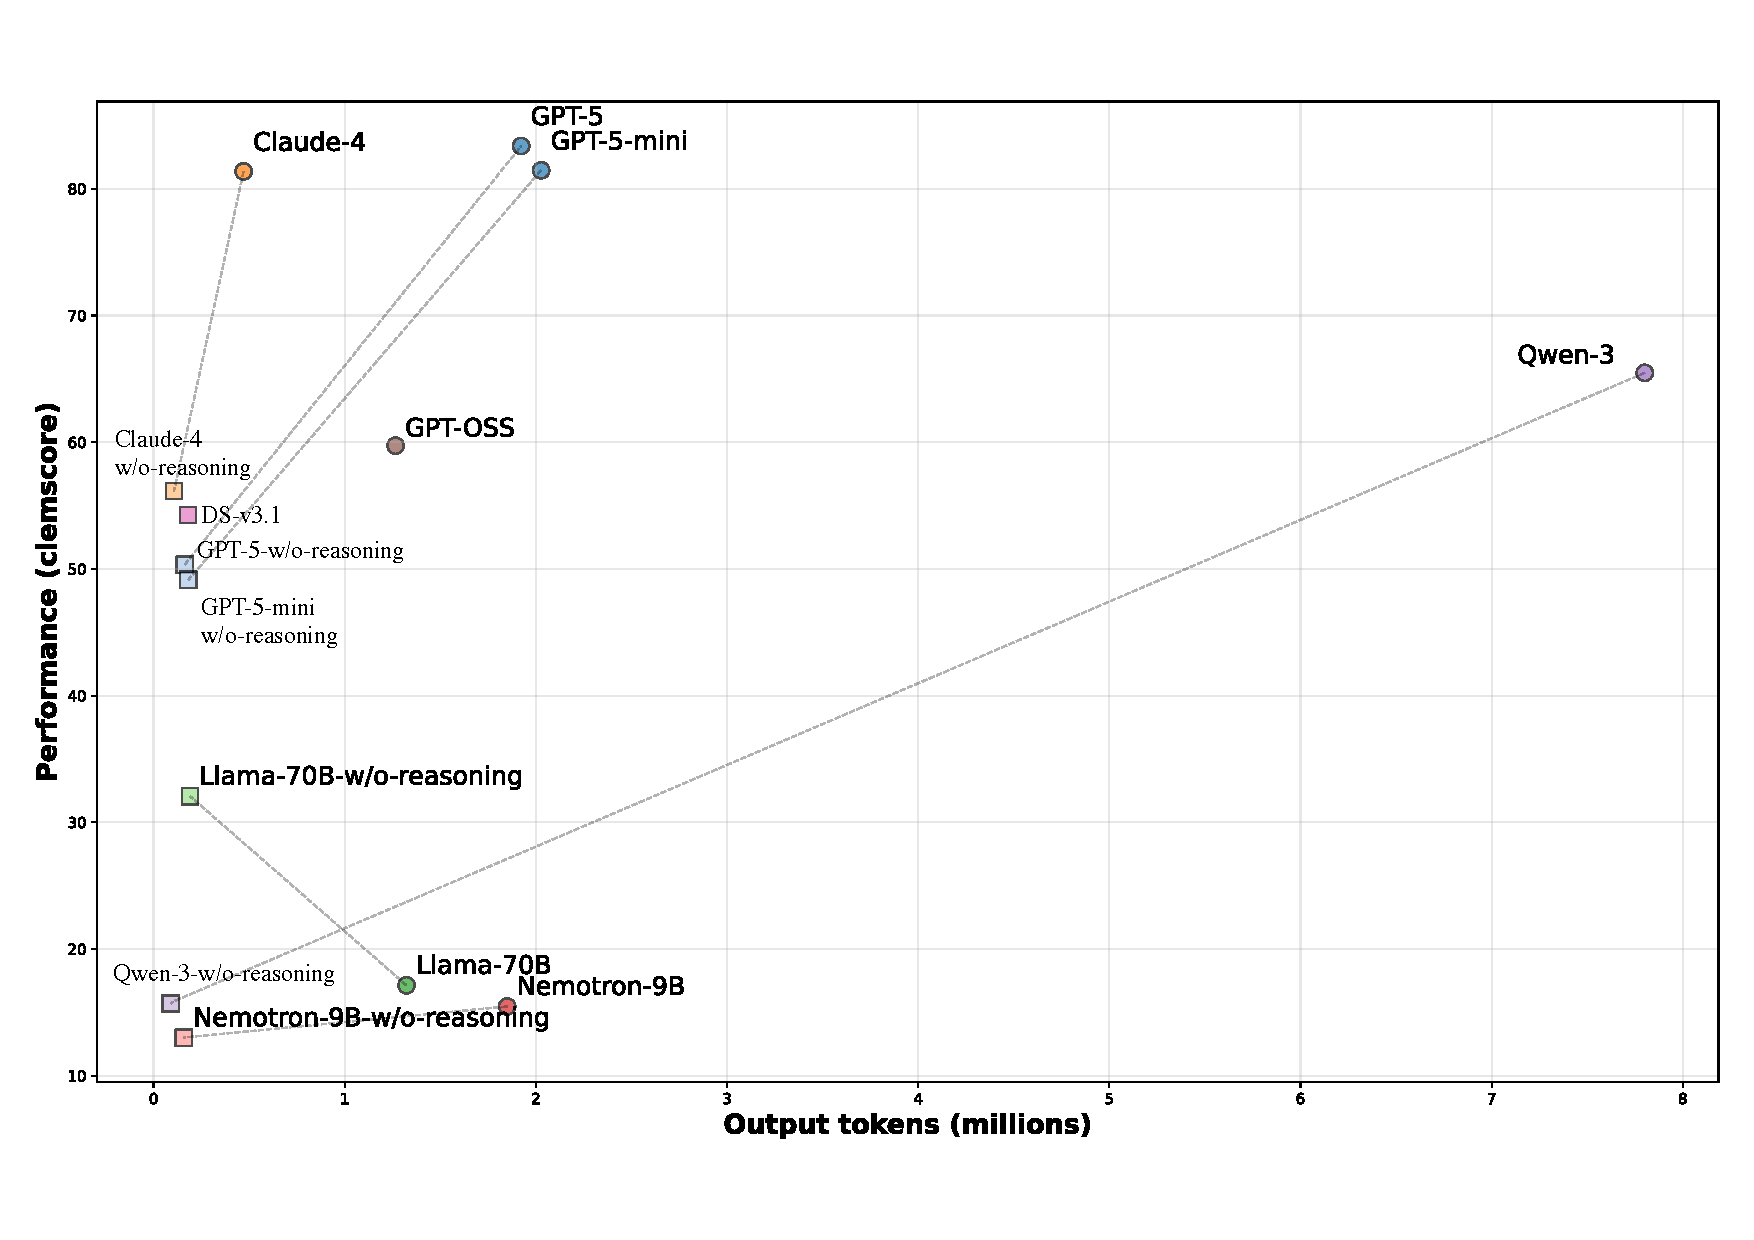
\includegraphics[width=\linewidth]{figures/token_plot_average.pdf}
        \caption{Average performance (clemscore) and the number of output tokens for all evaluated models with their reasoning on/off modes for English, German and Italian.}
        \label{fig:token_average}
    \end{subfigure}
    \hfill
    \begin{subfigure}[b]{0.48\textwidth}
        \centering
        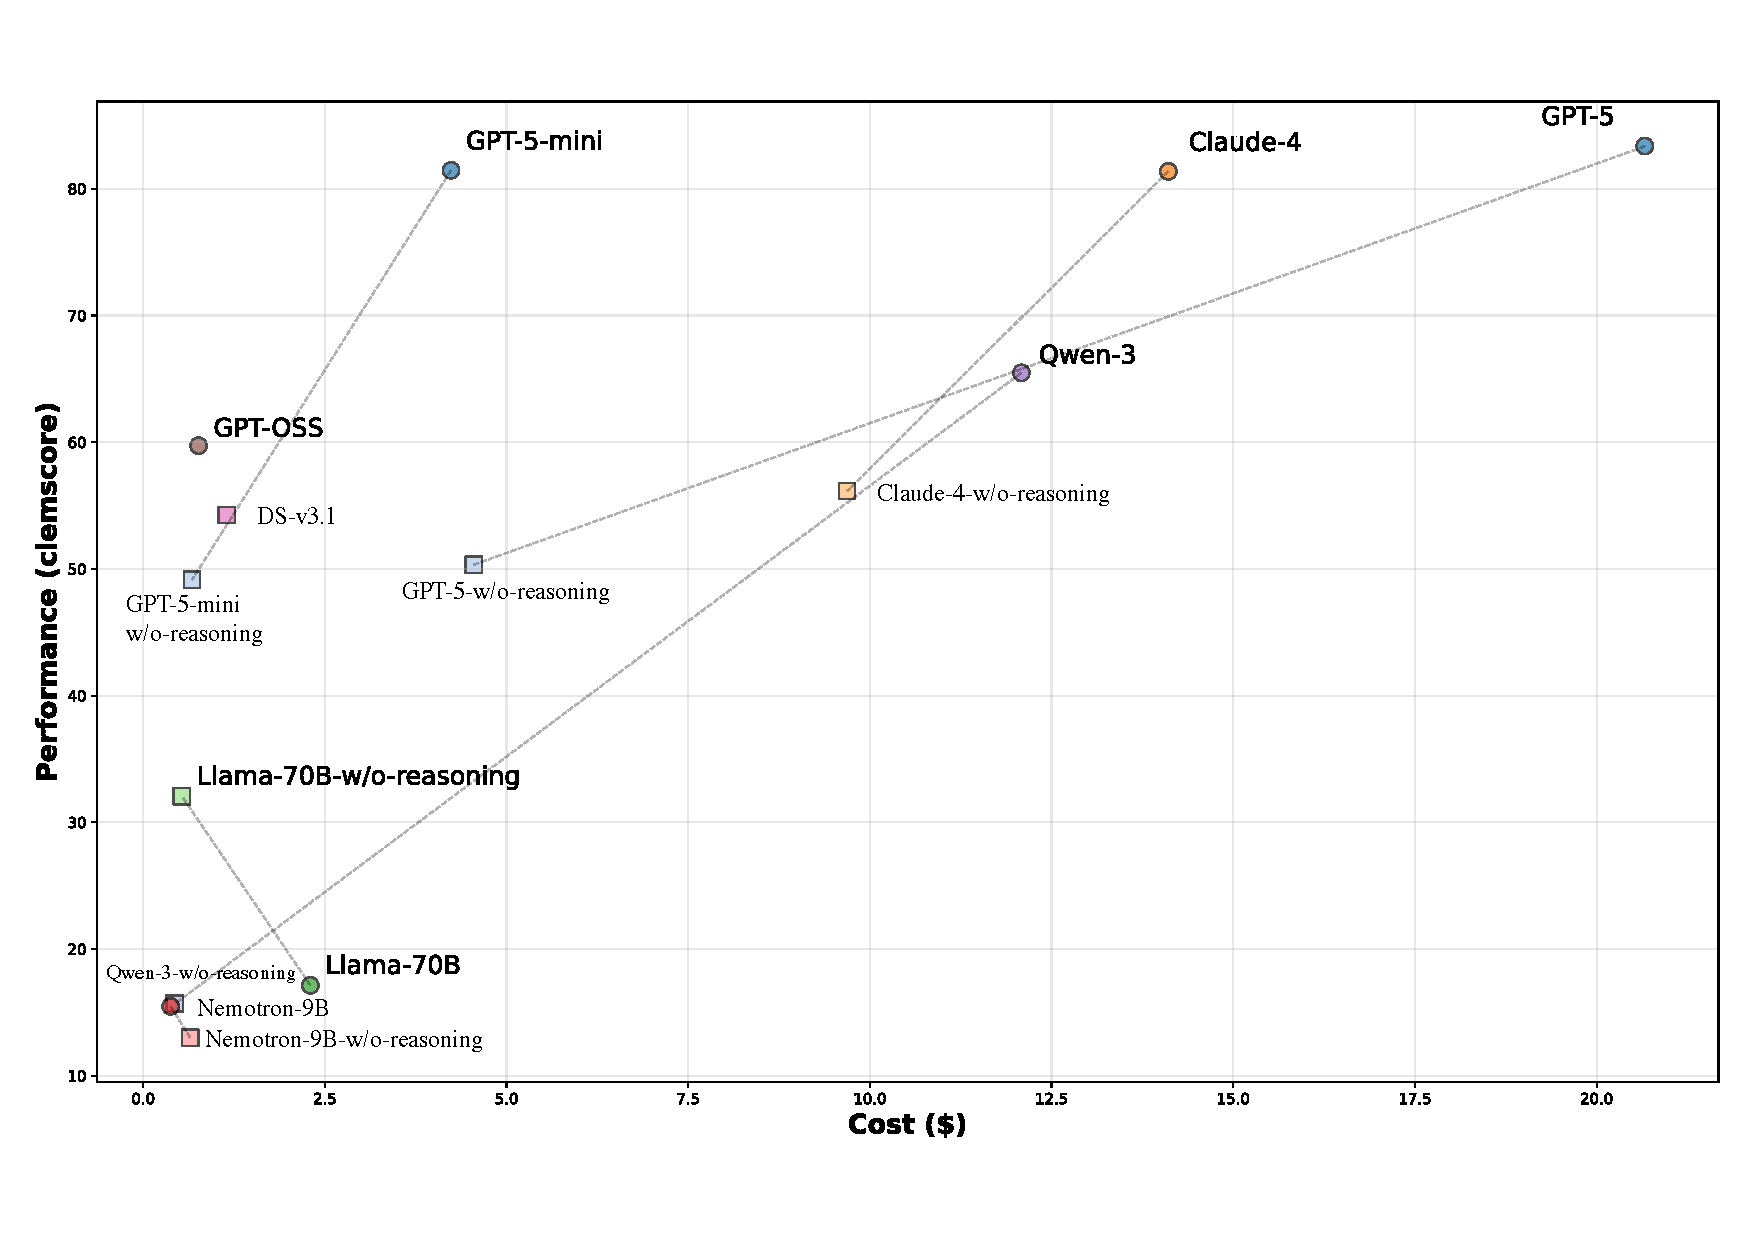
\includegraphics[width=\linewidth]{figures/cost_plot_average.pdf}
        \caption{Average performance (clemscore) and the cost of for all evaluated models with their reasoning on/off modes for English, German and Italian.}
        \label{fig:cost_average}
    \end{subfigure}
    \caption{Trade-off between performance and cost comparison across different models. Results for all languages are averaged.}
    \label{fig:combined}
\end{figure*}

% \begin{figure}[ht]
%     \centering
%     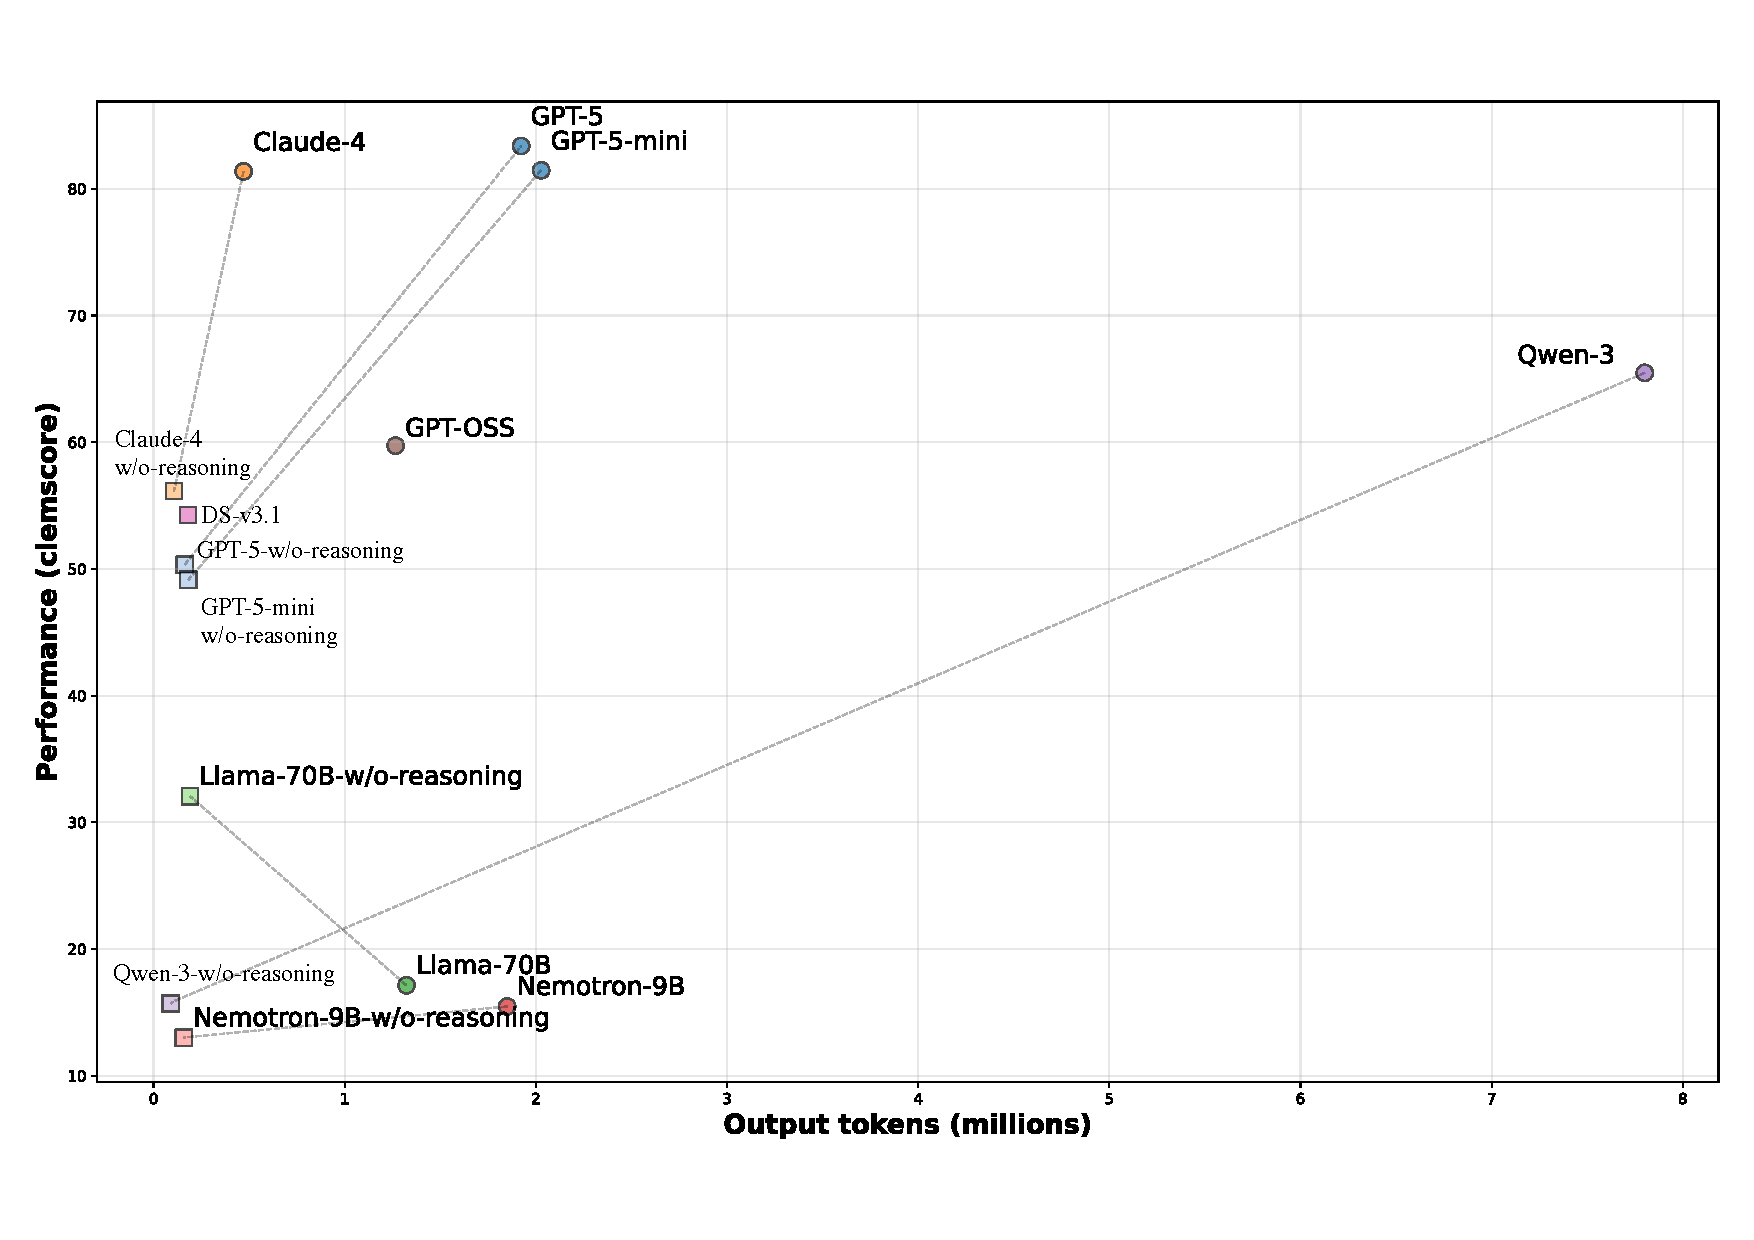
\includegraphics[width=1.0\linewidth]{figures/token_plot_average.pdf}
%     \caption{Average performance (clemscore) and the number of output tokens for all evaluated models with their reasoning on/off modes for English, German and Italian.}
%     \label{fig:token_average}
% \end{figure}

% \begin{figure}[ht]
%     \centering
%     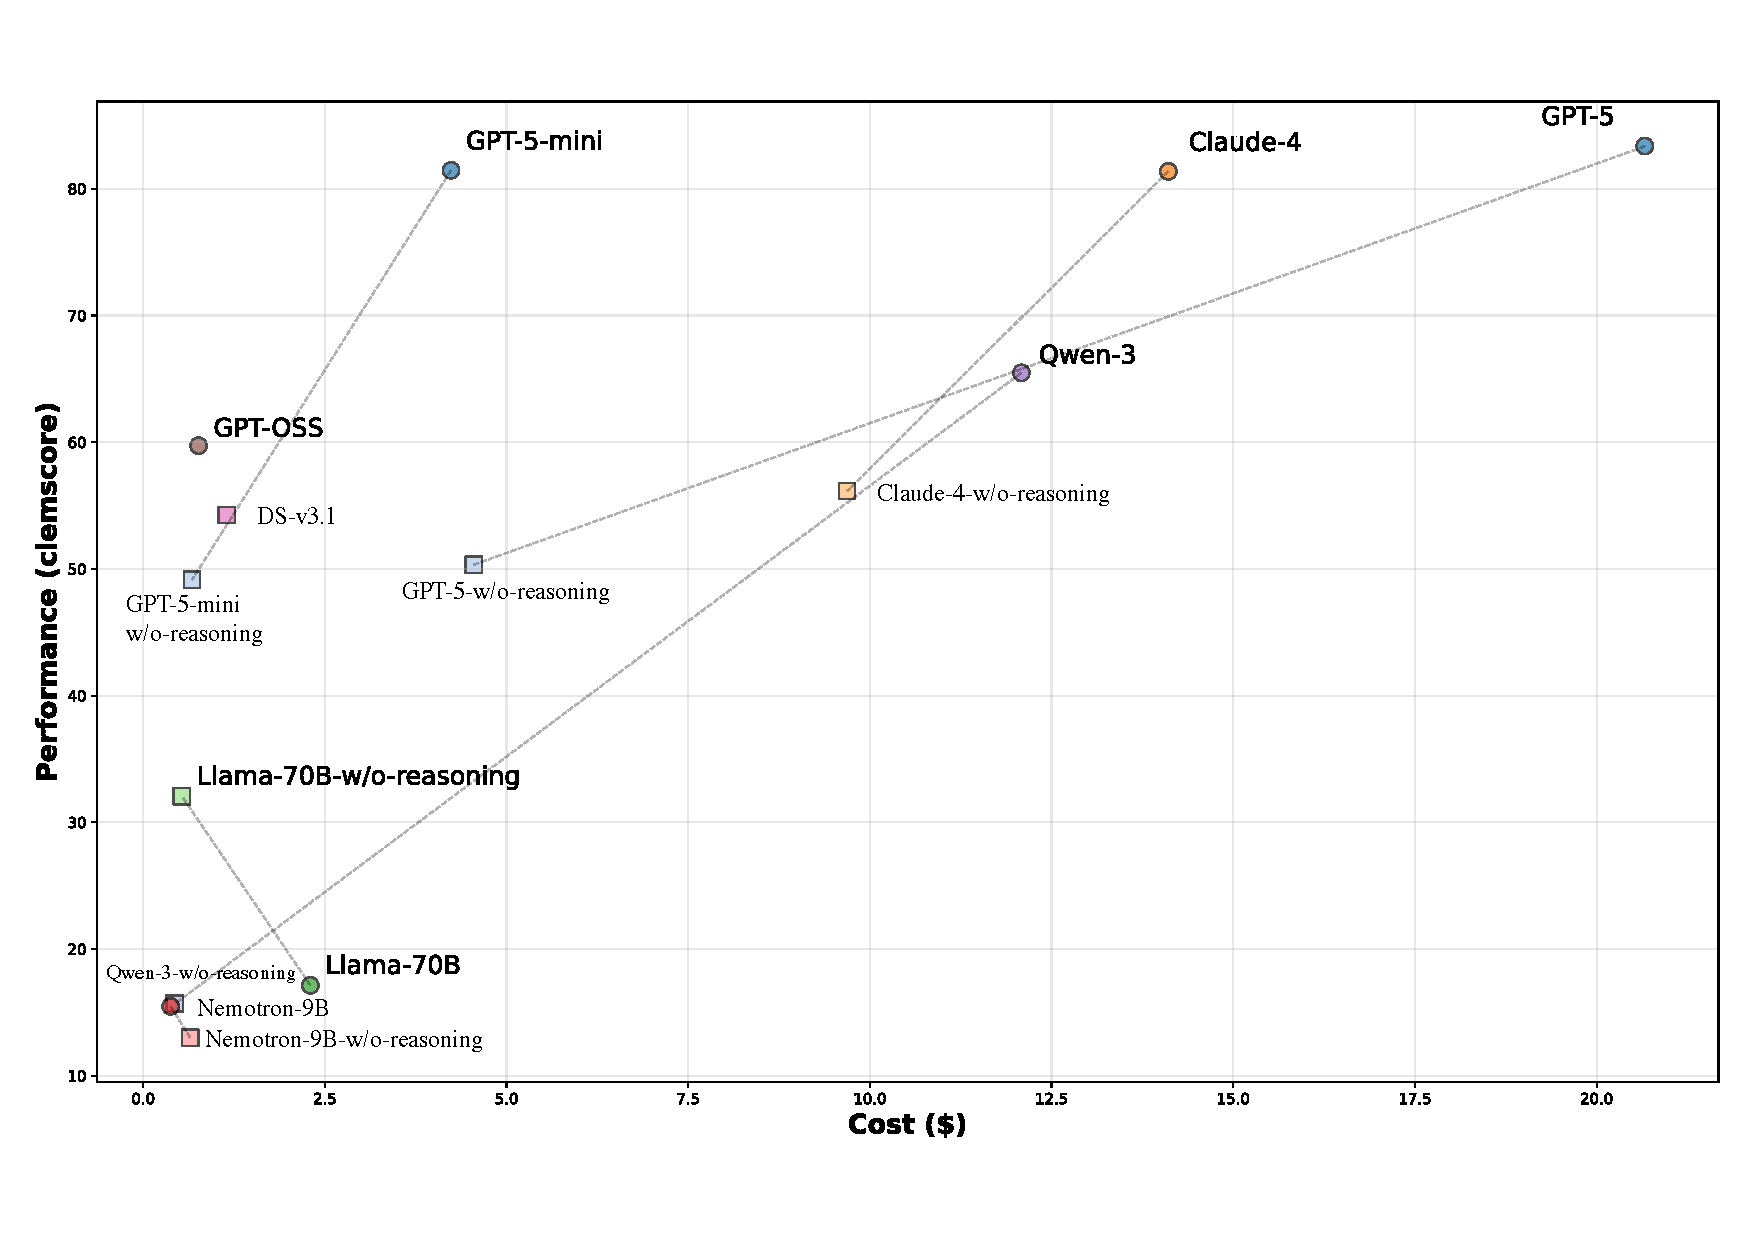
\includegraphics[width=1.0\linewidth]{figures/cost_plot_average.pdf}
%     \caption{Average performance (clemscore) and the cost of for all evaluated models with their reasoning on/off modes for English, German and Italian.}
%     \label{fig:cost_average}
% \end{figure}



\subsection{Qualitative Analysis}



\section{Conclusion}

\section*{Limitations}

LIMITATIONS

\newpage

%\bibliography{anthology,custom}
% Custom bibliography entries only
\bibliography{custom, anthology_0, anthology_1}

% \section*{Acknowledgments}




\appendix

\section{Additional Analysis}\label{sec:appendix_reamining_details}
\subfile{appendix/remainig_details}

\section{Deal or No Deal - Game Details}\label{sec:appendix_dond}
\subfile{dond/dond_appendix}


\section{Clean Up - Game Details}\label{sec:appendix_clean_up}
\subfile{clean_up/clean_up_appendix}

\section{Air Balloon Survival - Game Details}\label{sec:appendix_airballoon}
\subfile{air-balloon-survival/air_balloon_appendix}

\end{document}
